% Options for packages loaded elsewhere
\PassOptionsToPackage{unicode}{hyperref}
\PassOptionsToPackage{hyphens}{url}
%
\documentclass[
  english,
  man]{apa6}
\usepackage{amsmath,amssymb}
\usepackage{lmodern}
\usepackage{ifxetex,ifluatex}
\ifnum 0\ifxetex 1\fi\ifluatex 1\fi=0 % if pdftex
  \usepackage[T1]{fontenc}
  \usepackage[utf8]{inputenc}
  \usepackage{textcomp} % provide euro and other symbols
\else % if luatex or xetex
  \usepackage{unicode-math}
  \defaultfontfeatures{Scale=MatchLowercase}
  \defaultfontfeatures[\rmfamily]{Ligatures=TeX,Scale=1}
\fi
% Use upquote if available, for straight quotes in verbatim environments
\IfFileExists{upquote.sty}{\usepackage{upquote}}{}
\IfFileExists{microtype.sty}{% use microtype if available
  \usepackage[]{microtype}
  \UseMicrotypeSet[protrusion]{basicmath} % disable protrusion for tt fonts
}{}
\makeatletter
\@ifundefined{KOMAClassName}{% if non-KOMA class
  \IfFileExists{parskip.sty}{%
    \usepackage{parskip}
  }{% else
    \setlength{\parindent}{0pt}
    \setlength{\parskip}{6pt plus 2pt minus 1pt}}
}{% if KOMA class
  \KOMAoptions{parskip=half}}
\makeatother
\usepackage{xcolor}
\IfFileExists{xurl.sty}{\usepackage{xurl}}{} % add URL line breaks if available
\IfFileExists{bookmark.sty}{\usepackage{bookmark}}{\usepackage{hyperref}}
\hypersetup{
  pdftitle={Reproducing the analysis in Acute Effect of Physical Exercise on Negative Affect in Borderline Personality Disorder by Amour, Cailhol, and Ruocco},
  pdfauthor={Natalie Palmer1 \& Samuel St-Amour2},
  pdflang={en-EN},
  pdfkeywords={borderline personlaity, exercise},
  hidelinks,
  pdfcreator={LaTeX via pandoc}}
\urlstyle{same} % disable monospaced font for URLs
\usepackage{graphicx}
\makeatletter
\def\maxwidth{\ifdim\Gin@nat@width>\linewidth\linewidth\else\Gin@nat@width\fi}
\def\maxheight{\ifdim\Gin@nat@height>\textheight\textheight\else\Gin@nat@height\fi}
\makeatother
% Scale images if necessary, so that they will not overflow the page
% margins by default, and it is still possible to overwrite the defaults
% using explicit options in \includegraphics[width, height, ...]{}
\setkeys{Gin}{width=\maxwidth,height=\maxheight,keepaspectratio}
% Set default figure placement to htbp
\makeatletter
\def\fps@figure{htbp}
\makeatother
\setlength{\emergencystretch}{3em} % prevent overfull lines
\providecommand{\tightlist}{%
  \setlength{\itemsep}{0pt}\setlength{\parskip}{0pt}}
\setcounter{secnumdepth}{-\maxdimen} % remove section numbering
% Make \paragraph and \subparagraph free-standing
\ifx\paragraph\undefined\else
  \let\oldparagraph\paragraph
  \renewcommand{\paragraph}[1]{\oldparagraph{#1}\mbox{}}
\fi
\ifx\subparagraph\undefined\else
  \let\oldsubparagraph\subparagraph
  \renewcommand{\subparagraph}[1]{\oldsubparagraph{#1}\mbox{}}
\fi
% Manuscript styling
\usepackage{upgreek}
\captionsetup{font=singlespacing,justification=justified}

% Table formatting
\usepackage{longtable}
\usepackage{lscape}
% \usepackage[counterclockwise]{rotating}   % Landscape page setup for large tables
\usepackage{multirow}		% Table styling
\usepackage{tabularx}		% Control Column width
\usepackage[flushleft]{threeparttable}	% Allows for three part tables with a specified notes section
\usepackage{threeparttablex}            % Lets threeparttable work with longtable

% Create new environments so endfloat can handle them
% \newenvironment{ltable}
%   {\begin{landscape}\centering\begin{threeparttable}}
%   {\end{threeparttable}\end{landscape}}
\newenvironment{lltable}{\begin{landscape}\centering\begin{ThreePartTable}}{\end{ThreePartTable}\end{landscape}}

% Enables adjusting longtable caption width to table width
% Solution found at http://golatex.de/longtable-mit-caption-so-breit-wie-die-tabelle-t15767.html
\makeatletter
\newcommand\LastLTentrywidth{1em}
\newlength\longtablewidth
\setlength{\longtablewidth}{1in}
\newcommand{\getlongtablewidth}{\begingroup \ifcsname LT@\roman{LT@tables}\endcsname \global\longtablewidth=0pt \renewcommand{\LT@entry}[2]{\global\advance\longtablewidth by ##2\relax\gdef\LastLTentrywidth{##2}}\@nameuse{LT@\roman{LT@tables}} \fi \endgroup}

% \setlength{\parindent}{0.5in}
% \setlength{\parskip}{0pt plus 0pt minus 0pt}

% \usepackage{etoolbox}
\makeatletter
\patchcmd{\HyOrg@maketitle}
  {\section{\normalfont\normalsize\abstractname}}
  {\section*{\normalfont\normalsize\abstractname}}
  {}{\typeout{Failed to patch abstract.}}
\patchcmd{\HyOrg@maketitle}
  {\section{\protect\normalfont{\@title}}}
  {\section*{\protect\normalfont{\@title}}}
  {}{\typeout{Failed to patch title.}}
\makeatother
\shorttitle{Exercise on Negative Affect in BPD}
\keywords{borderline personlaity, exercise\newline\indent Word count: X}
\DeclareDelayedFloatFlavor{ThreePartTable}{table}
\DeclareDelayedFloatFlavor{lltable}{table}
\DeclareDelayedFloatFlavor*{longtable}{table}
\makeatletter
\renewcommand{\efloat@iwrite}[1]{\immediate\expandafter\protected@write\csname efloat@post#1\endcsname{}}
\makeatother
\usepackage{lineno}

\linenumbers
\usepackage{csquotes}
\ifxetex
  % Load polyglossia as late as possible: uses bidi with RTL langages (e.g. Hebrew, Arabic)
  \usepackage{polyglossia}
  \setmainlanguage[]{english}
\else
  \usepackage[main=english]{babel}
% get rid of language-specific shorthands (see #6817):
\let\LanguageShortHands\languageshorthands
\def\languageshorthands#1{}
\fi
\ifluatex
  \usepackage{selnolig}  % disable illegal ligatures
\fi
\newlength{\cslhangindent}
\setlength{\cslhangindent}{1.5em}
\newlength{\csllabelwidth}
\setlength{\csllabelwidth}{3em}
\newenvironment{CSLReferences}[2] % #1 hanging-ident, #2 entry spacing
 {% don't indent paragraphs
  \setlength{\parindent}{0pt}
  % turn on hanging indent if param 1 is 1
  \ifodd #1 \everypar{\setlength{\hangindent}{\cslhangindent}}\ignorespaces\fi
  % set entry spacing
  \ifnum #2 > 0
  \setlength{\parskip}{#2\baselineskip}
  \fi
 }%
 {}
\usepackage{calc}
\newcommand{\CSLBlock}[1]{#1\hfill\break}
\newcommand{\CSLLeftMargin}[1]{\parbox[t]{\csllabelwidth}{#1}}
\newcommand{\CSLRightInline}[1]{\parbox[t]{\linewidth - \csllabelwidth}{#1}\break}
\newcommand{\CSLIndent}[1]{\hspace{\cslhangindent}#1}

\title{Reproducing the analysis in Acute Effect of Physical Exercise on Negative Affect in Borderline Personality Disorder by Amour, Cailhol, and Ruocco}
\author{Natalie Palmer\textsuperscript{1} \& Samuel St-Amour\textsuperscript{2}}
\date{}


\affiliation{\vspace{0.5cm}\textsuperscript{1} Brooklyn College of the City University of New York\\\textsuperscript{2} Department of Psychology (Scarborough), University of Toronto}

\abstract{
The study was conducted by St-Amour, S., Cailhol, L., Ruocco, A. C., \& Bernard, P.(2021, April 1). The origional paper can be found at \url{https://osf.io/preprints/sportrxiv/mdcuh/}

This study looks at exercise as a potential strategy to reduce negative affect in individuals with borderline personality disorder. Negative affect was induced in all participants and they were randomly assigned to either an experimental or control condition. Affect was measured using a feeling scale and arousal scale before and after mood induction.

This is a reproduction of the repeated measures t-test performed to assess the negative mood induction strategy used by the researchers.
The induction strategy had a significant effect on inducing negative feeling in participants. However, there was not a significant difference in arousal ratings before and after the induction strategy.
}



\begin{document}
\maketitle

\hypertarget{introduction}{%
\section{Introduction}\label{introduction}}

This report reproduces the repeated measures t-test used to evaluate the effectiveness of the negative mood induction strategy performed in the experiment by Amour et al.~(2021). Open data can be downloaded from \url{https://osf.io/t2egx/}.

This goal of this study was to see whether or not exercise could be a beneficial emotion regulation strategy for individuals with borderline personality disorder (BPD). All participant had to go through a negative mood induction procedure which consisted of watching a short scene from The Silence of the Lambs which has been shown to induce negative feelings in individuals with borderline personality. After the negative mood induction, participants were randomly assigned into an exercise condition which consisted of 20 minutes of physical exercise on a stationary bike, or a control condition which consisted of watching a 20 minute clip from a ``neutral'' film. The researchers used ``The Feeling Scale'' (FS) to measure affective valence with a range from -5(very bad) to 5(very good). They also used ``The Felt Arousal Scale'' (FAS) to measure arousal, which ranged from 1 (low arousal) to 6 (high arousal).

\hypertarget{methods}{%
\section{Methods}\label{methods}}

Researchers used ``The Felt Arousal Scale'' (FAS; Svebak and Murgatroyd, 1985) and ``The Feeling Scale'' (FS; Hardy and Rejeski, 1989) to measure participants general feeling before and after the negative induction strategy.

\hypertarget{participants}{%
\subsection{Participants}\label{participants}}

Participants in the study were recruited from the Personality and Relational Disorders Services from the Mental Health University Institute of Montreal. The study consisted of 27 participants, all of whom were diagnosed with borderline personality disorder.

\hypertarget{procedure}{%
\subsection{Procedure}\label{procedure}}

Participants all had to go through a negative mood induction strategy which was watching a scene from Silence of the Lambs. Researchers measured negative and positive valence as well as arousal in all participants seven times throughout the experiment. Before the negative mood induction strategy, right before the induction strategy, immediately following the negative mood induction, 5 minutes into the experimental condition, 10 minutes into the experimental condition, 15 minutes into the experimental condition, and at the end of he experiment.

\hypertarget{data-analysis}{%
\subsection{Data analysis}\label{data-analysis}}

\hypertarget{results}{%
\section{Results}\label{results}}

Feeling and arousal scores were collected directly before and immediately after the negative mood induction strategy. A repeated measures t-test was used to look at effectiveness of the strategy in both.

\hypertarget{repeated-measures-t-test-for-feeling-scores-before-and-after}{%
\section{Repeated Measures T-Test for Feeling Scores before and after}\label{repeated-measures-t-test-for-feeling-scores-before-and-after}}

The participants feeling scores (FS) were significantly more negative after (M = -0.2592593, SD = 2.58) the scence from Silence of the Lambs than before ( M = 5.074, SD = 2.52678), t(26) = 2.41, df = 26, p-value = 0.023. The mean difference was ( M = 1.59)

\hypertarget{repeated-measures-t-test-for-arousal-scores-before-and-after}{%
\section{Repeated Measures T-Test for Arousal Scores before and after}\label{repeated-measures-t-test-for-arousal-scores-before-and-after}}

However, the participants arousal scores were not significantly more negative (FAS) after (M = 6.81, SD = 2.527) the scence from Silence of the Lambs than before ( M = 5.074, SD = 2.525), t(26) = -3.2845, df = 26, p-value = 0.00292. The mean difference was ( M = -1.740741 )

apa\_print(means\_df)

\begin{verbatim}
## 
##  Paired t-test
## 
## data:  arousal_feeling_scores$feeling_before and arousal_feeling_scores$feeling_after
## t = 2.4102, df = 26, p-value = 0.02332
## alternative hypothesis: true difference in means is not equal to 0
## 95 percent confidence interval:
##  0.2343307 2.9508544
## sample estimates:
## mean of the differences 
##                1.592593
\end{verbatim}

\begin{verbatim}
## 
##  Paired t-test
## 
## data:  arousal_feeling_scores$arousal_before and arousal_feeling_scores$arousal_after
## t = -3.2845, df = 26, p-value = 0.00292
## alternative hypothesis: true difference in means is not equal to 0
## 95 percent confidence interval:
##  -2.8301531 -0.6513284
## sample estimates:
## mean of the differences 
##               -1.740741
\end{verbatim}

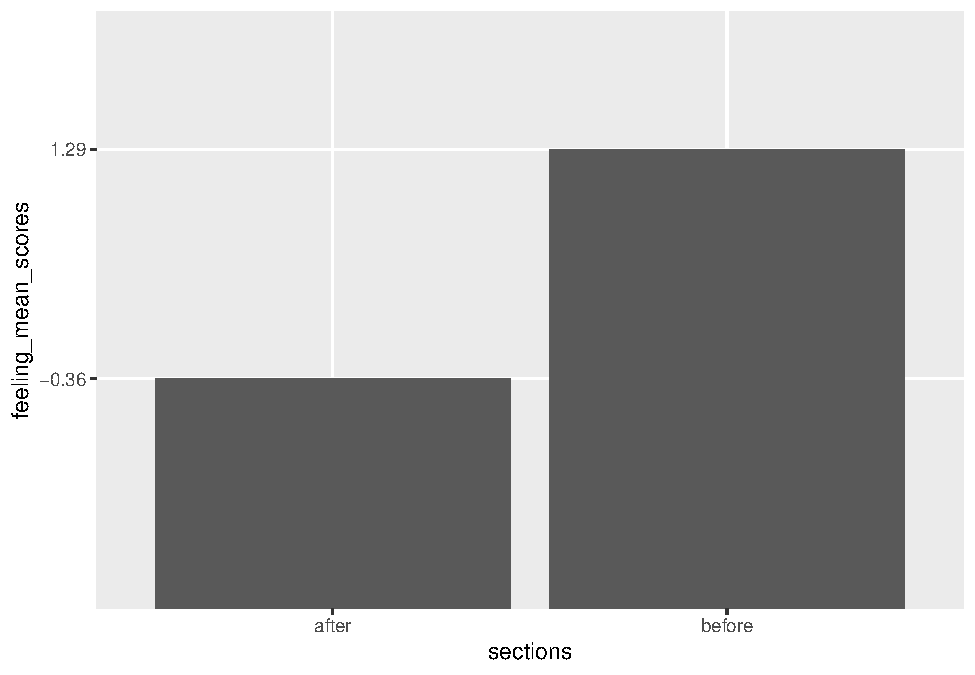
\includegraphics{APAReport_files/figure-latex/unnamed-chunk-1-1.pdf}

\hypertarget{discussion}{%
\section{Discussion}\label{discussion}}

The re-analysis somewhat successfully reproduced the analysis reported by (\textbf{st-amour\_cailhol\_ruocco\_bernard\_2021?}). My results for the repeated measures t-test looking at feeling scores were the same (my means for before and after scores slightly varied). However, my results for the t test that looked at arousal before and after were not the same.

The researchers reported:

The valence of feeling scores were significantly more negative (FS) after (M = -0.36, SD = 2.59)
the scene from Silence of the Lambs than before (M = 1.29, SD = 2.49), t(26) = 2.41, p = .023, d =
0.46, but the clip did not impact the arousal (FAS), t(26) = -1.79, p = .086

\hypertarget{power-analysis}{%
\section{Power Analysis}\label{power-analysis}}

The following reports a power curve analysis for the t-test with 27 participants. This shows the power of the design to detect effects of different sizes.

This experiment had 27 subjects. The results of the power curve are shown below. When the effect size is around 1.0 a design of this nature will detect that effect at the .05 level nearly 100 percent of the time. I do believe that this study could have benefited from a slightly larger sample size.

apa\_print(plot\_df)

\begin{figure}
\centering
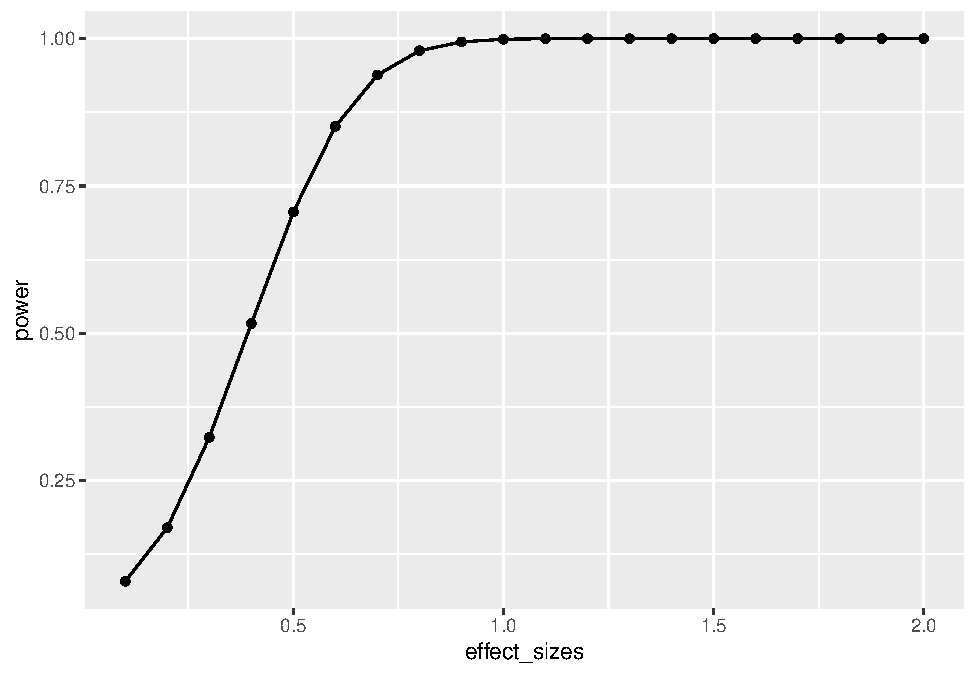
\includegraphics{APAReport_files/figure-latex/unnamed-chunk-2-1.pdf}
\caption{\label{fig:unnamed-chunk-2}A Power curve for a t-test with 27 participants}
\end{figure}

\newpage

\hypertarget{references}{%
\section{References}\label{references}}

St-Amour, S., Cailhol, L., Ruocco, A. C., \& Bernard, P. (2021, April 1). Acute Effect
of Physical Exercise on Negative Affect in Borderline Personality Disorder: A Pilot Study.
\url{https://doi.org/10.31236/osf.io/mdcuh}

\{r create\_r-references\}
r\_refs(file = ``r-references.bib'')

\begingroup
\setlength{\parindent}{-0.5in}
\setlength{\leftskip}{0.5in}

\hypertarget{refs}{}
\begin{CSLReferences}{0}{0}
\end{CSLReferences}

\endgroup


\end{document}
